\chapter{Build Your own EMG (2A)}

Now that we know how to build an opamp circuit to amplify a signal, we can build our own Electromyography circuit.  You probably noticed how sensitive the opamp circuits were to the resistor values, so we will use a specialized device called an instrumentation amplifier, which is designed to amplify weak signals by combining non-inverting amplifiers with precision matched resistances referenced to each other through a gain resistor (which controls the gain of both) that feeds into a differential amplifier setup (like an inverting amplifier of one signal with respect to a voltage divided version of the second).

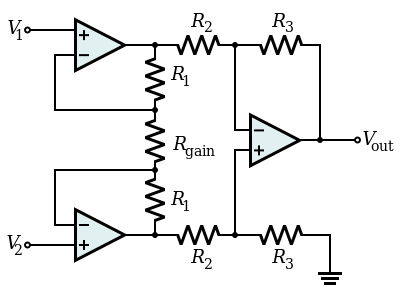
\includegraphics[width=0.4\textwidth]{../images/400px-Op-Amp_Instrumentation_Amplifier.png}

\section{Wiring the Circuit}

We are using an Analog Devices 8221 (AD8221) instrumentation amplifier, that is on a breakout board.  The breakout board contains resistors and capacitors needed to make the circuit run well.  For instance the positive and negative rails have a capacitor to ground that is used to clean up the power.  Additionally, the positive and negative inputs have 4k$\Omega$ resistors inline and a capacitor to ground - which acts like a low pass filter.  Finally, the gain resistor is set at 499$\Omega$ to make the gain about 100.  The breakout board greatly simplifies our lives by providing a nicely set up system.  The input impedance is a bit low for us, but it will work.  If you add more resistance on the inputs, it will reduce the corner frequency of the low pass filter and cause other issues, so we will just leave it.  The signal will need extra amplification so we will run the output into two inverting amplifier stages (each side of our current LM358 opamp) and then to the 3008 and then to our PI.  The first stage will get gain of 100, which makes the total gain 10000 times, but since the input is loaded and weak, we will need a second stage with a gain of 25, then we should get a nice signal.  The overall circuit we will build is below.  Note the red lines and components are the instrumentation amplifier breakout board, so you don't need to add each component, just the board.

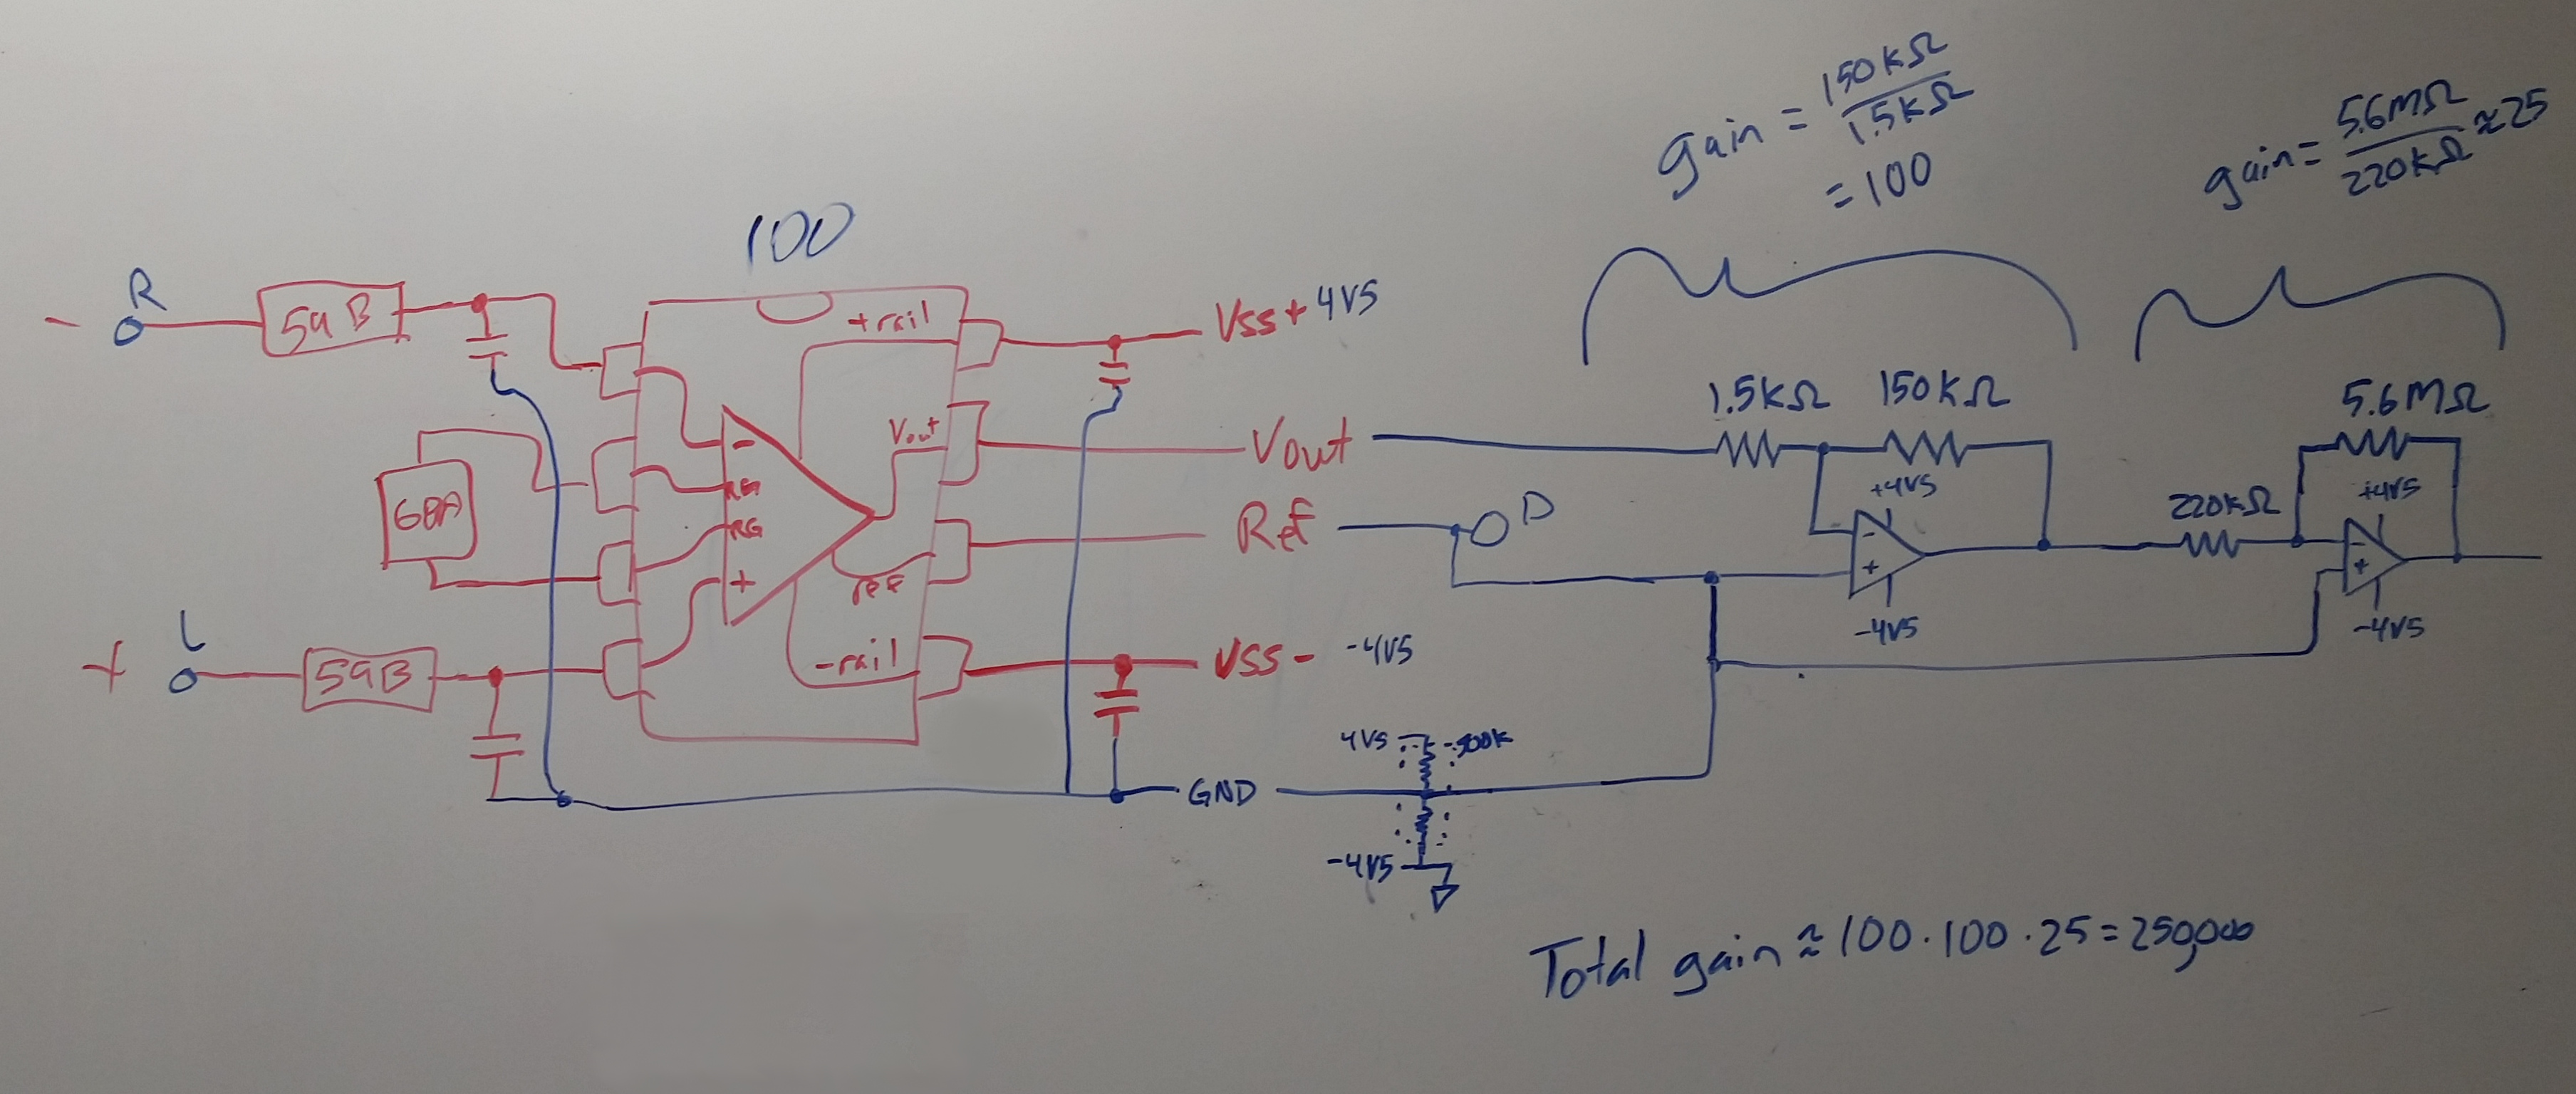
\includegraphics[width=\textwidth]{../images/EMG_complete.jpg}

To get the gain of 100, we need to set the resistor between the output of the first stage (pin 1 of our opamp) and the negative input (pin 2 of the opamp) to be 100 times the resistance of the one between the negative input and signal from the instrumentation amplifiers output.  We will set the impedance to be a moderate range using 150k$\Omega$ and  1.5k$\Omega$ respectively.  %Note if we need to dial the gain back we can replace the 150k$\Omega$ resistor with one side (either side to the center tap) of the 500k$\Omega$ potentiometer.

The second stage needs around a gain of 25, and we will pick the impedance to be around a mega ohm, so that we can easily set up a filter with a corner frequency around 100 Hz if we need to.  Thus we will pick the resistor between the output (pin 6 of the opamp) and the negative input (pin 5 of the opamp) to be 5.6M$\Omega$ and the resistor from the negative input and the output of the first stage (pin 1 of the opamp) to be 220k$\Omega$.  Note: I tested a number of the instrumentation amps and some needed 33ok$\Omega$ resistor instead of 220k$\Omega$, because the gain was too high for the dc component.  If you get clipping you can reduce the gain by swapping the 220k$\Omega$ resistor for a 330k$\Omega$ resistor.  The output of the entire circuit is from pin 6 of the opamp.  The net connection diagram is below.

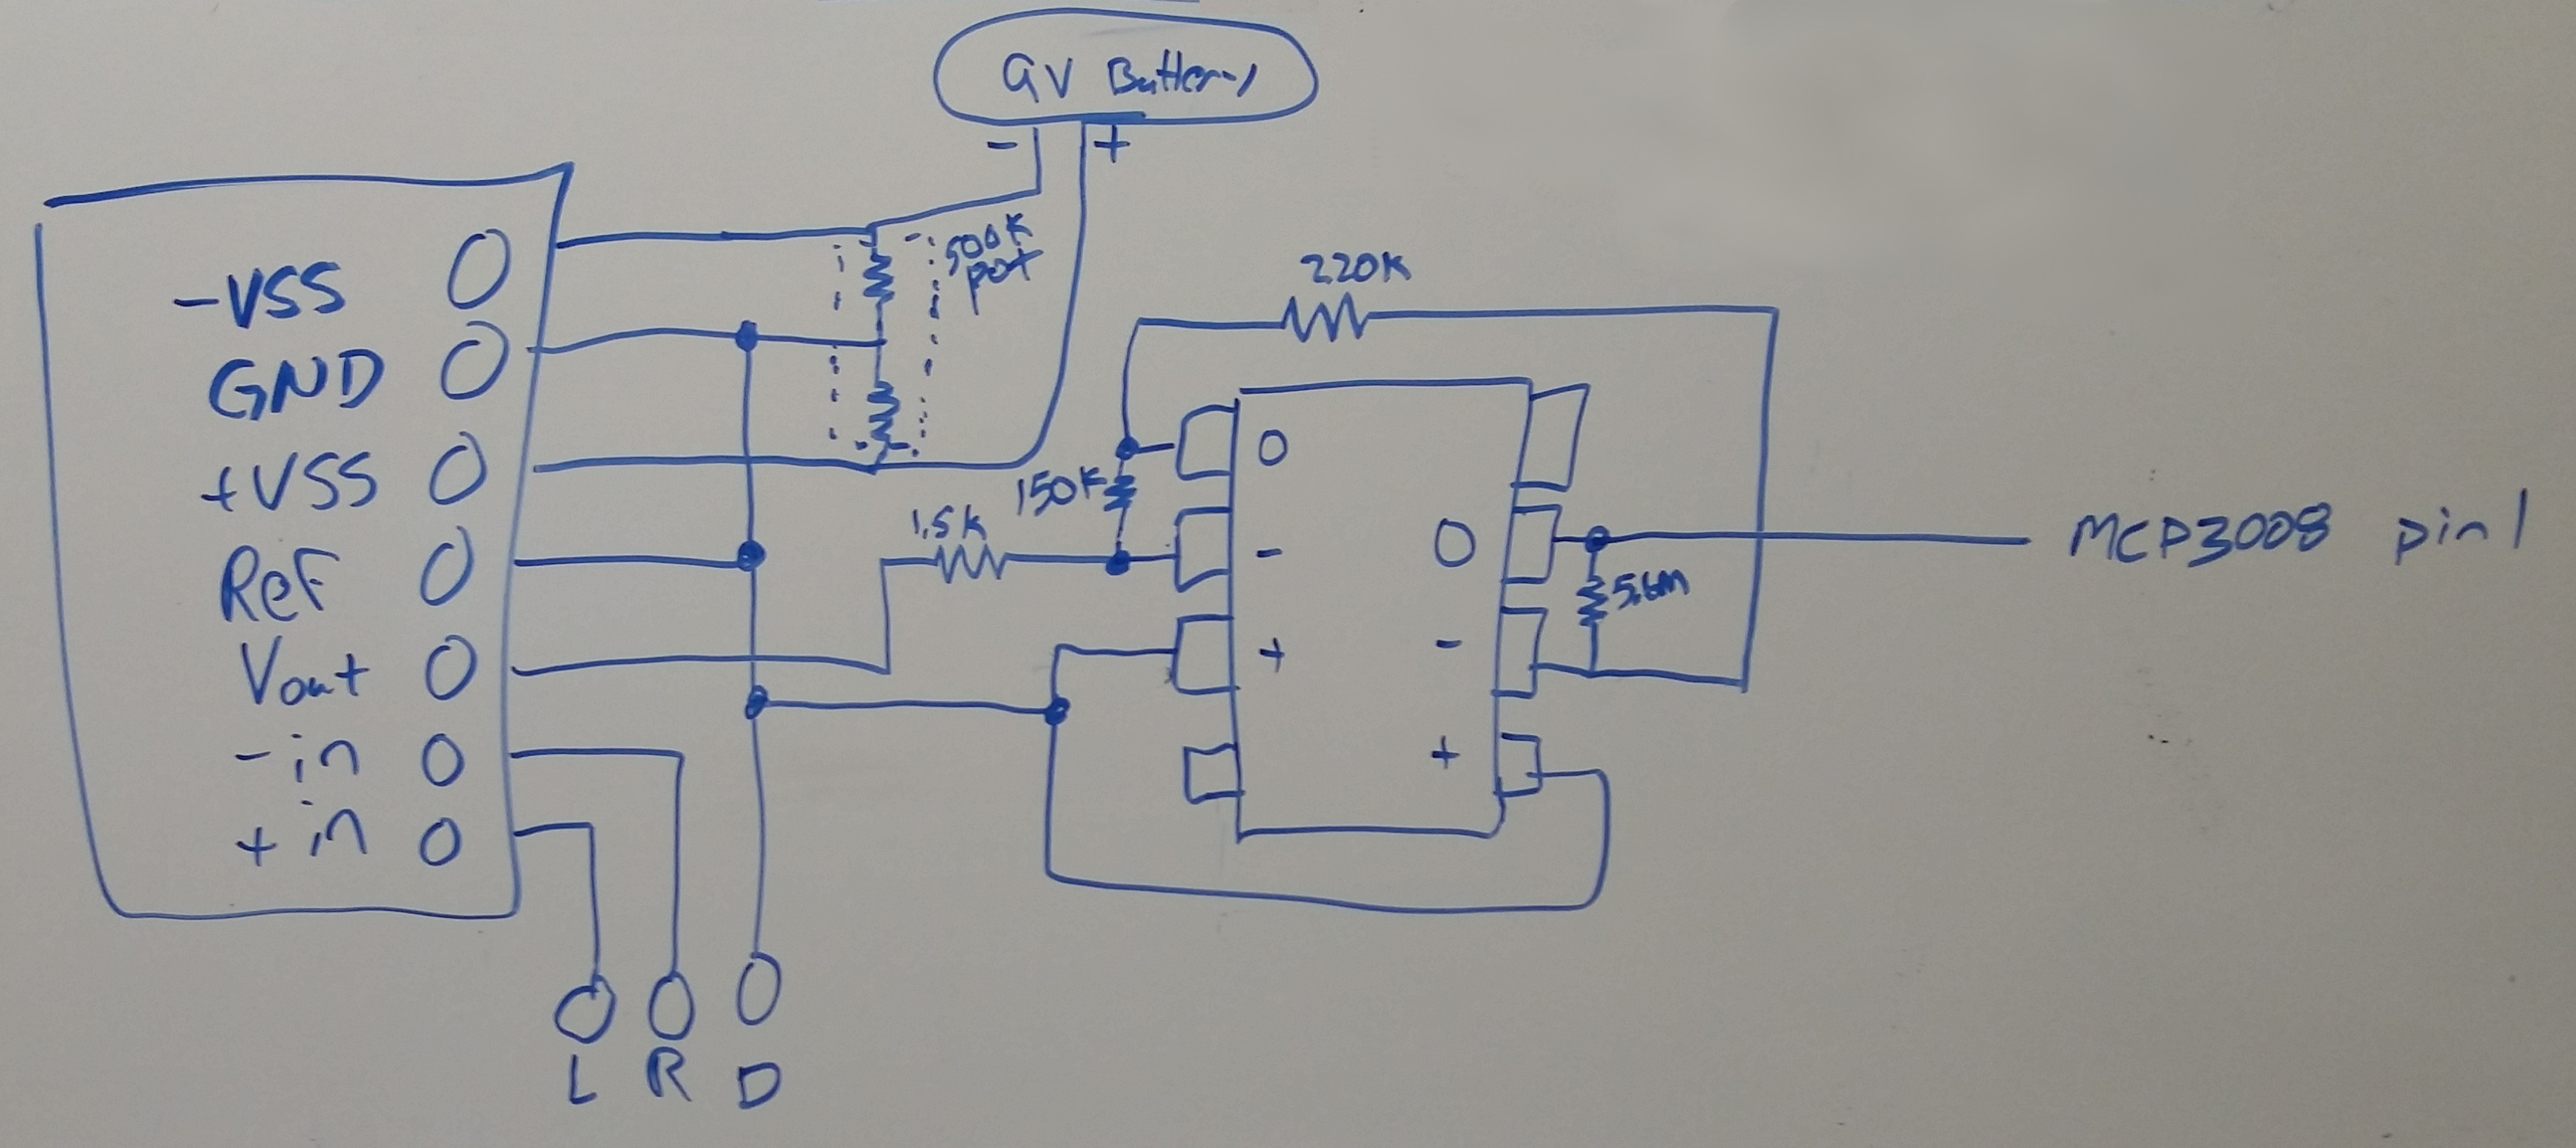
\includegraphics[width=\textwidth]{../images/EMG_connect.jpg}

The positive and negative rail will be powered by a 9v battery. This will do two things:
\begin{enumerate}
\item you will be isolated from wall power, greatly increasing your safety.
\item the circuit will have a bigger voltage swing, which will make the amplifier's job much easier.
\end{enumerate}
We will connect the negative battery lead to the Raspberry Pi's ground\footnote{In a commercial circuit we would put this through a large resistor or an isolator.  We can't do that for R and L, since they tuned the 4k$\$Omega$ input to their capacitors, so if we put another resistor to bring it to the 80k$\Omega$ plus range it would change the low pass filter (LPF) to have a significantly reduced corner frequency and thus additional noise.  The setup we are using should only be used for EMG on the same arm with people who don't have a pacemaker. In extreme circumstances such as a lightning strike to ground current could come back from the ground and short a component redirecting current to any of the leads.  The amount of current to cause problems is lower if the heart is between any of the probes (hence only use for one arm) and even more with arrythmia that requires a pacemaker or similar.} We will make a false ground for the instrumentation amp using the 500k potentiometer and the 9v battery, setting the false ground around 1.4 volts.  Note the audio connector has the following pinout, so you can connect it.


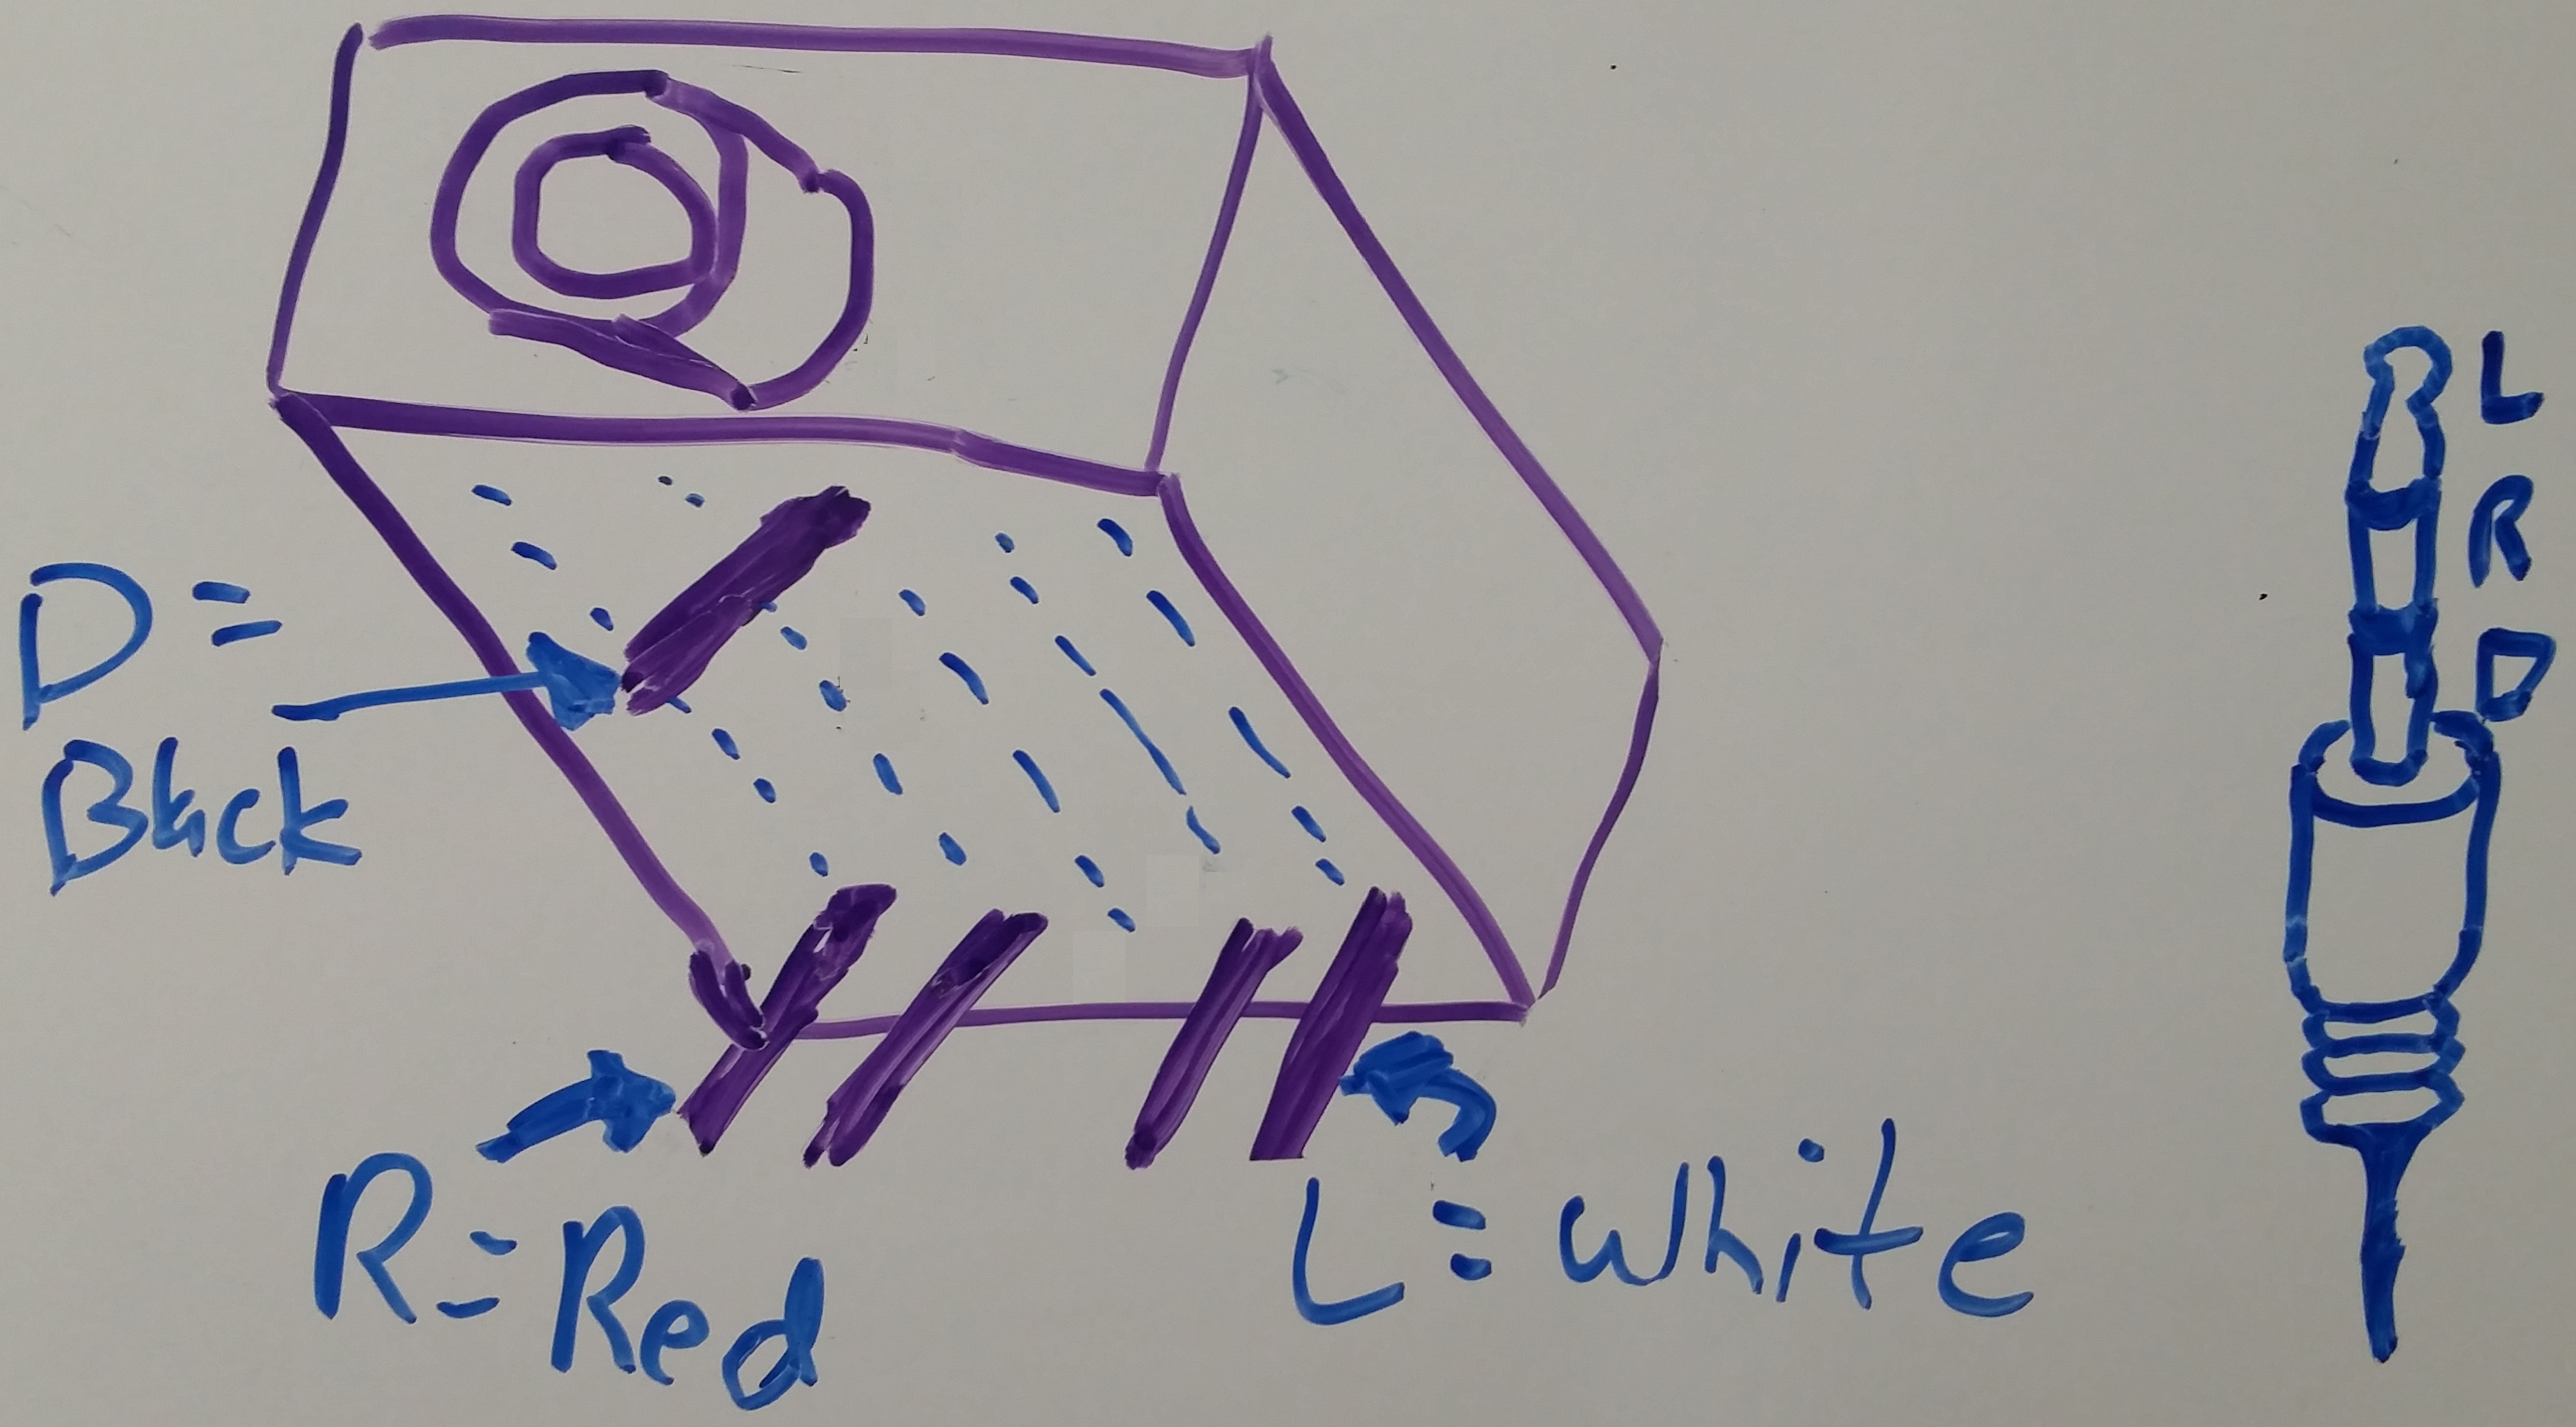
\includegraphics[width=.3\textwidth]{../images/audio_jack.jpg}

\section{Graphing}

This circuit is much more power hungry than the simple circuits we used, and so you will notice a difference in the plotting efficency, since the Raspberry Pi will run slower.  To counter this we need to go to a more efficient piece of code.  Our current code uses one thread that takes in data and plots.  It is more efficient to make two threads - one that takes in data and puts it in the array, and one that just plots data.  This is implemented in the MCP3008thread[1-4].py code.  The first two are more generic, while the third is special of our case - it plots one line and has our values preset, and saves a file with the data when you exit, so use it.  The fourth takes a fixed count of 20000 data points so you can save the figure.

\CommandLine{cd c*/B*/l*/*3}

\CommandLine{sudo python MCP3008plot_thread3.py}

Plot the data for the same muscle group you did on the EMG shield and compare how easy it is to make out the muscle contractions.  Compare the quality of the two circuits.

\section{Optional Reference: Understanding the AD8221 Breakout}

\noindent
\begin{tabular}{cc}
Bottom & Top \\
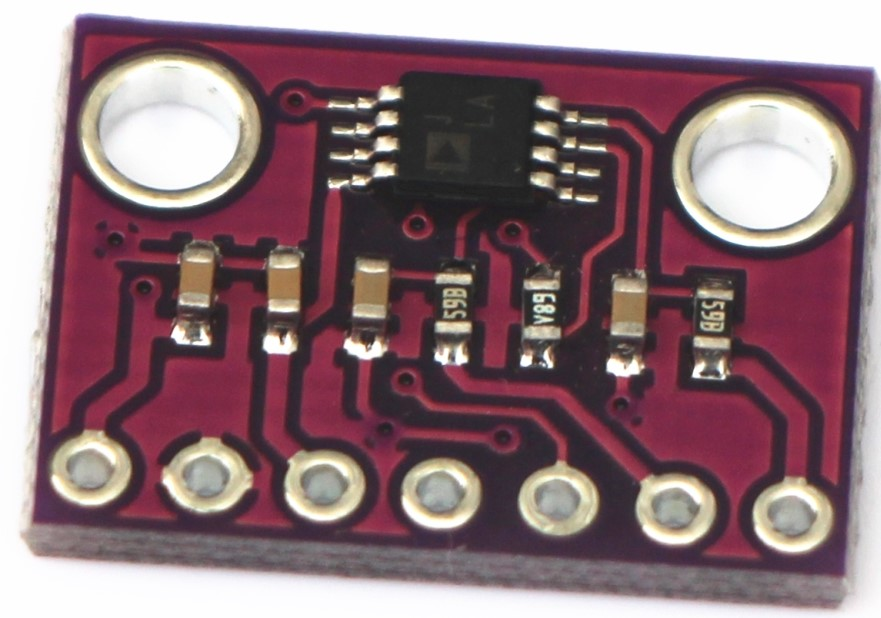
\includegraphics[width=0.3\textwidth]{../images/InstAmpBreakoutBottom.jpg} &
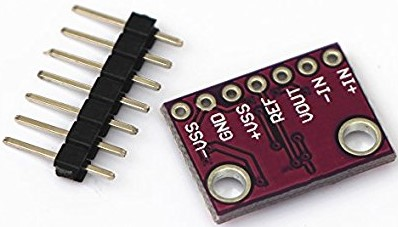
\includegraphics[width=0.5\textwidth]{../images/InstAmpBreakoutTop.jpg}\\
\end{tabular}

The AD8221 instrumentation amplifier pinout is

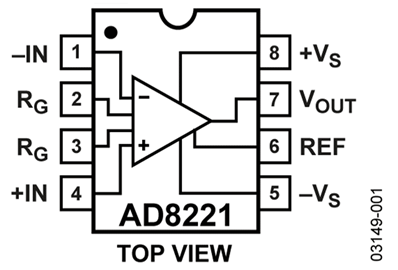
\includegraphics[width=0.38\textwidth]{../images/AD8221-FBL.png}

Surface mount resistors have three potential codes: 3 numbers, 4 numbers, and EIA-96.  The board uses E96 resistors (1\% tolerance) and thus uses the EIA-96 Codes.  The first two numbers are a code you look up (see first chart) to get the 3 digit value of the resistor, and the Letter at the end is the multiplier (see second chart).

\noindent
\begin{tabular}{ll||ll||ll||ll||ll||ll}
Code    & Value	& Code	& Value	& Code	& Value	& Code	& Value	& Code	& Value	& Code	& Value\\\hline\hline
01      & 100	& 17	& 147	& 33	& 215	& 49	& 316	& 65	& 464	& 81	& 681\\
02      & 102	& 18	& 150	& 34	& 221	& 50	& 324	& 66	& 475	& 82	& 698\\
03      & 105	& 19	& 154	& 35	& 226	& 51	& 332	& 67	& 487	& 83	& 715\\\hline
04      & 107	& 20	& 158	& 36	& 232	& 52	& 340	& 68	& 499	& 84	& 732\\
05      & 110	& 21	& 162	& 37	& 237	& 53	& 348	& 69	& 511	& 85	& 750\\
06      & 113	& 22	& 165	& 38	& 243	& 54	& 357	& 70	& 523	& 86	& 768\\\hline
07      & 115	& 23	& 169	& 39	& 249	& 55	& 365	& 71	& 536	& 87	& 787\\
08      & 118	& 24	& 174	& 40	& 255	& 56	& 374	& 72	& 549	& 88	& 806\\
09      & 121	& 25	& 178	& 41	& 261	& 57	& 383	& 73	& 562	& 89	& 825\\\hline
10      & 124	& 26	& 182	& 42	& 267	& 58	& 392	& 74	& 576	& 90	& 845\\
11      & 127	& 27	& 187	& 43	& 274	& 59	& 402	& 75	& 590	& 91	& 866\\
12      & 130	& 28	& 191	& 44	& 280	& 60	& 412	& 76	& 604	& 92	& 887\\\hline
13      & 133	& 29	& 196	& 45	& 287	& 61	& 422	& 77	& 619	& 93	& 909\\
14      & 137	& 30	& 200	& 46	& 294	& 62	& 432	& 78	& 634	& 94	& 931\\
15      & 140	& 31	& 205	& 47	& 301	& 63	& 442	& 79	& 649	& 95	& 953\\\hline
16      & 143	& 32	& 210	& 48	& 309	& 64	& 453	& 80	& 665	& 96	& 976\\
\end{tabular}

\noindent
\begin{tabular}{ll}
Code	& Multiply factor\\ \hline
Z       & 0.001\\
Y/R	    & 0.01\\
X/S	    & 0.1\\
A       & 1\\
B/H	    & 10\\
C       & 100\\
D       & 1,000\\
E       & 10,000\\
F       & 10,0000\\
\end{tabular}
